\documentclass[a0paper,portrait]{baposter}

\usepackage{bm}
\usepackage{tikz}
\usepackage{color}
\usepackage{xcolor}
\usepackage{enumitem}
\usepackage[]{apacite}
%\usepackage{multicol} 
\usepackage{wrapfig}
\usepackage{lmodern}
\usepackage{amsmath}
\usepackage{amssymb}
\usepackage{graphicx}
\usepackage{tabularx}
\usepackage{listings}
\usepackage{colortbl}
\usepackage[T1]{fontenc}
\usepackage{stackengine}
\usepackage[utf8]{inputenc} %unicode support
\usepackage{mathtools, nccmath}

%%
%\usepackage[style=ieee]{biblatex}
%\addbibresource{gpBias.bib}
%
%natbib
%\renewcommand{\bibsection}{}
%
%\usepackage{etoolbox}
%\patchcmd{\thebibliography}{\section*{\refname}}{}{}{}

\usetikzlibrary{positioning, shapes, snakes}

\selectcolormodel{cmyk}

%\graphicspath{{figures/}} % Directory in which figures are stored


\newcommand{\compresslist}{%
\setlength{\itemsep}{0pt}%
\setlength{\parskip}{1pt}%
\setlength{\parsep}{0pt}%
}

\newenvironment{boenumerate}
  {\begin{enumerate}\renewcommand\labelenumi{\textbf\theenumi.}}
  {\end{enumerate}}

\newcommand{\redhat}[1]{\color{red}\hat{\text{$#1$}}}
\newcommand{\orangebar}[1]{\color{orange}\bar{\text{$#1$}}}

%
\begin{document}

%
\definecolor{darkgreen}{cmyk}{0.8,0,0.8,0.45}
\definecolor{lightgreen}{cmyk}{0.8,0,0.8,0.25}
\definecolor{darkblue}{HTML}{000080}%{1A5276}%{2471A3}
\definecolor{lightblue}{HTML}{0000FF}%{2E86C1}
\definecolor{black}{HTML}{000000}
\definecolor{violet}{HTML}{8000FF}

%
\begin{poster}
{
grid=false,
headerborder=open, % Adds a border around the header of content boxes
colspacing=1em, % Column spacing
bgColorOne=white, % Background color for the gradient on the left side of the poster
bgColorTwo=white, % Background color for the gradient on the right side of the poster
borderColor=lightblue, % Border color
headerColorOne=lightblue, % Background color for the header in the content boxes (left side)
headerColorTwo=lightblue, % Background color for the header in the content boxes (right side)
headerFontColor=white, % Text color for the header text in the content boxes
boxColorOne=white, % Background color of the content boxes
textborder=rounded, %rectangle, % Format of the border around content boxes, can be: none, bars, coils, triangles, rectangle, rounded, roundedsmall, roundedright or faded
eyecatcher=false, % Set to false for ignoring the left logo in the title and move the title left
headerheight=0.11\textheight, % Height of the header
headershape=rounded, % Specify the rounded corner in the content box headers, can be: rectangle, small-rounded, roundedright, roundedleft or rounded
headershade=plain,
headerfont=\Large\textsf, % Large, bold and sans serif font in the headers of content boxes
%textfont={\setlength{\parindent}{1.5em}}, % Uncomment for paragraph indentation
linewidth=2pt % Width of the border lines around content boxes
}
{}
%
%TITLE
%
{
\vspace{3cm}
\begin{minipage}{0.14\textwidth}
	
\includegraphics[width=1\textwidth]{./noaa.jpeg}
\end{minipage}
\begin{minipage}{0.7\textwidth}
	%\vspace*{-3cm}
	%\hspace*{1cm}
	\begin{center}					%Fisheries
	{\huge \textbf{A Metamodel Based Clustering of Production Model Reference Point Estimation.}}\\ 
	\vspace{0.5cm}
	{\Large Nick Grunloh$^a$, E.J. Dick$^b$, and Herbie Lee$^a$}
	\end{center}
\end{minipage}
\begin{minipage}{0.14\textwidth}
	\hspace*{-0.5cm}
	
\includegraphics[width=1.2\textwidth]{./fiatSlug.jpg}
\end{minipage}
\normalsize
\\ \sf
$^a$ Department of Statistical Science, Baskin School of Engineering, University of California Santa Cruz, 1156 High Street, Santa Cruz, CA 95064, USA\\
$^b$ Fisheries Ecology Division, Southwest Fisheries Science Center, National Marine Fisheries Service, NOAA, 110 McAllister Way, Santa Cruz, CA 95060, USA\\
}
\\

%
\headerbox{Abstract}{name=introduction,column=0,row=0.06,span=3}{
Integrated fisheries models are based upon differential equations which model
stock dynamics through time. Fisheries are largely managed based upon
quantities derived from the equilibrium equations of these dynamics, known as
Reference Points (RP). RP behavior is primarily driven by the functional form
of the productivity assumed in the differential equations. \shortciteA{mangel_perspective_2013} %Mangel et. al. (2013) 
demonstrate that the most commonly used models of productivity limit the
domain of RPs due to a lack of flexibility induced by their two-parameter
functional forms. Three-parameter models of production release this theoretical
RP limitation \shortcite{punt_extending_2019}. %(Punt \& Cope, 2019). 
Nonetheless, two-parameter models of
productivity are overwhelmingly used in practice. When RP model misspecification
of this type is present in population dynamics models, what are the useful limits
of statistical inference with respect to estimating these RPs? Here, a simulation
environment is designed which explores how misspecified two-parameter production
models bias RP inference. Using a Gaussian Process metamodel of the inferred RPs
(under two-parameter productivity), the full theoretical space of RP bias
behavior is explored. This structured simulation setting allows for clustering
of RP failure modes which use the metamodel to predict when a given species is
most likely to be subject to catastrophic model failure.
%Effective management of exploited fish populations requires accurate estimates
%of commercial fisheries catches to inform monitoring and assessment efforts. In
%California, the high degree of heterogeneity in the species composition of many
%groundfish fisheries, particularly those targeting rockfish (genus Sebastes), 
%leads to challenges in sampling all potential strata, or species, adequately. 
%Limited resources and increasingly complex stratification of the sampling system 
%inevitably leads to gaps in sample data. In the presence of sampling gaps, 
%current methods for speciating commercial landings provide ad-hoc point estimates 
%of species compositions in unsampled strata by “borrowing” data across adjacent 
%stratum in time and space. Due to complex interactions between biogeography and
%market category sorting dynamics, it is not possible to be certain about optimal 
%a’priori pooling strategies. Here we introduce a Bayesian Model Averaging (BMA) 
%method for discovering quantitatively justifiable pooling strategies by averaging 
%across exhaustive sets of spatially partitioned models. In combination with Bayesian 
%hierarchical modeling, these methods allow us to infer pooling strategies from port 
%sampling data. Furthermore, these methods allow for a complete statistical summary 
%of several of the most important sources of uncertainty. 
}

%1. Model
\headerbox{1. Fisheries Production Model}{name=model,column=0,below=introduction,span=2}{
	%
        \begin{minipage}[h!]{0.45\textwidth}	
	%
	\begin{equation*}
	I_t = q B_t e^\epsilon ~~~ \epsilon\sim N(0, \sigma^2)
	\end{equation*}
	%
	\subsubsection*{Population Dynamics:}
	\begin{align*}
	&\medmath{\frac{dB}{dt}} \medmath{= \overbrace{w(a_s)R(B_{t-a_s})}^\text{Recruitment} + \overbrace{\kappa \left[w_\infty N-B\right]}^\text{Net Growth} - \overbrace{(M+F)B}^\text{Mortality}} \\%\label{bEq}\\
	&\medmath{\frac{dN}{dt}} \medmath{= R(B_{t-a_s}) - (M+F)N} %\\%\label{nEq}\\
	%&~\\
	%&R(B_{t-a_s}; \theta): \text{Two v. Three Parameter}\\
	%&w(a) : \text{Individual Growth}
	\end{align*}
	%	
	\subsubsection*{Individuals Grow:}
	\centering
	\includegraphics[width=0.85\textwidth]{../../ddBias/vbPoster.png}
	%
        \end{minipage}
        \begin{minipage}[h!]{0.55\textwidth}
	%
	\subsubsection*{Recruitment Into the Population:}
	%{\color{red}
	%\begin{equation*}
	%R(B_{t-a_s}; \theta): \text{Two v. Three Parameter}	
	%\end{equation*}
	%Nonlinear.\\
	%Primary driver of RPs.\\
	%Two parameter limits to line and Three parameter expands space.	
	%}
	%
        \begin{minipage}[b]{0.5\textwidth}
        %$~$\\\vspace*{-10cm}
	\begin{itemize}[leftmargin=*]
		\raggedright	
		\item $R$ is notoriously nonlinear and unknown.%\makebox[\linewidth][l]{$R$ is nonlinear and unknown.}
		%\item Three parameter model shown right.
		\item Most models assume two-parameter $R_{(\alpha, \beta, -1)}$ 
		\item Fixing $\gamma$ limits RPs \& freeing $\gamma$ expands RPs.	
		\item $R_{(\alpha, \beta, \gamma)}$ $\gamma\in(-2,1)$ $\rightarrow$ %\\ Although a three parameter  
		%\item Fixing $\gamma$ limits RPs.
		%\item Fixing $\gamma=-1$ (black curve) is most common.%ly used model.
		%\item Two v. Three Parameter
		%\item Most models assume $\gamma=-1$
		 %Two parameter limits to line
		%\item {\color{red} Words can fix all things in time}
	\end{itemize}
	$~$\\$~$\\$~$\\
	\end{minipage}
	\begin{minipage}[b]{0.48\textwidth}
		$~$\\
		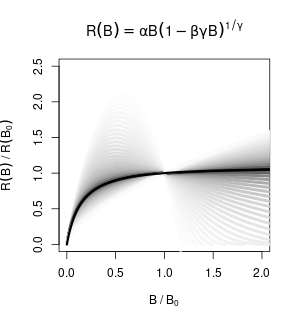
\includegraphics[width=\textwidth]{../../ddBias/g3Grey.png}
		$~$\\$~$\\
	\end{minipage}
	
	%
	\vspace*{-2cm}
	\subsubsection*{Reference Points: $\frac{F_{MSY}}{M}, ~\frac{B_{MSY}}{B_0}$}
	
	%%
	%\begin{align*}
        %\frac{F_{MSY}}{M}, ~\frac{B_{MSY}}{B_0}
        %\end{align*}		
	
	%
        \begin{minipage}[b]{0.5\textwidth}
	\begin{itemize}[leftmargin=*]
		\raggedright
		\item Measures of Maximum \mbox{Sustainable Yield ($MSY$)}
		\item Fishing Rate and Biomass Depletion. %at $MSY$. %mortality ata fraction of natural mortality
		%\item Biomass Depletion
		%\item $\frac{F_{MSY}}{M}, ~\frac{B_{MSY}}{B_0}$
		%\item Equilibrium quantities from dynamics.
		\item Primarily driven by $R$ and parameters $\alpha$, $\beta$, $\gamma$.
		%\item Inferred by learning $\alpha$, $\beta$, and $\gamma$ as possible. %from data.
                \item RPs are the foundation of mangement action.
        \end{itemize}
	$~$\\$~$\\$~$\\
	\end{minipage}
        \begin{minipage}[b]{0.48\textwidth}
	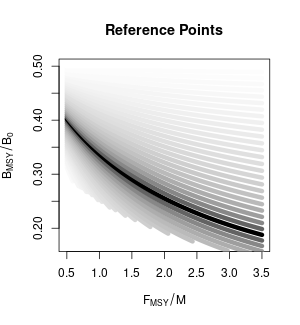
\includegraphics[width=\textwidth]{../../ddBias/rpCurves.png} %designLineColorHHardFlatT30N150WWideN112.png}
	$~$\\$~$\\$~$\\
	\end{minipage}
	$~$\vspace*{-1.75cm}
	%%
        %%\begin{center}
        %%$~$\\$~$\\$~$\\$~$\\$~$\\$~$\\$~$\\$~$\\
        %\hspace{-2cm}
        %\begin{tikzpicture}[overlay]
        %\node at (1,0) {\includegraphics[width=1\textwidth]{../../gpBias/designLineHHardExpT45N150M0.3Wide.pn
        %\node[circle, draw, minimum size=7, inner sep=-2] at (2.6,1.5){\tiny S};
        %\draw[latex-, very thick,black] (0.4,-1.1) -- ++(2,2.4);
        %\node[circle,fill=red, minimum size=9, inner sep=-2] at (0.25,-1.25){\tiny BH};
        %\end{tikzpicture}
        %%\end{center}
        %%$~$\\$~$\\$~$\\$~$\\$~$\\$~$\\$~$\\
	%%%
        \end{minipage}
}

%3. Bayesian Model Averaging
\headerbox{2. Simulation \& Metamodeling}{name=sim,column=2,below=introduction,span=1}{
	%
	Datasets are simulated broadly in RP space and fit with a misspecified two-parameter $R(B)$. 
	Two-parameter $R(B)$ induces bias in RPs by limiting estimates to the curve $\frac{1}{x+2}$. 
	Each data-set produces an example of the bias mapping. 	
	%\begin{center}
	%
	\begin{center}
	$~$\\$~$\\$~$\\$~$\\$~$\\%$~$\\%$~$\\%$~$\\
	\hspace{-2cm}
	\begin{tikzpicture}[overlay]
	\node at (1,0) {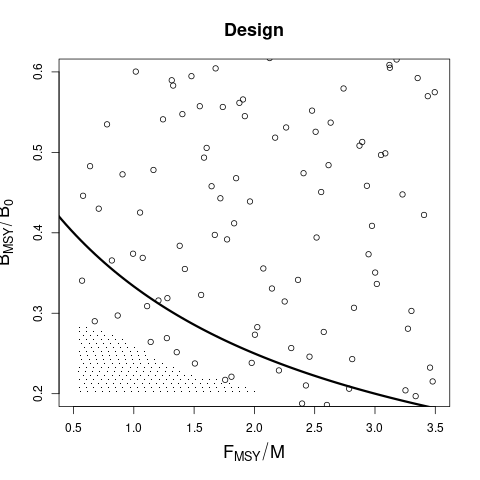
\includegraphics[width=0.69\textwidth]{../../gpBias/designLineHHardExpT45N150M0.3Wide.png}};
	\node[circle, draw, minimum size=7, inner sep=-2] at (2.4,1.4){\tiny 3};
	\draw[latex-, very thick,black] (0.8,-0.85) -- ++(1.45,2.1);
	\node[circle,fill=red, minimum size=9, inner sep=-2] at (0.7,-1){\tiny 2};
	\end{tikzpicture}
	\end{center}
	$~$\\$~$\\$~$\\$~$\\%$~$\\%$~$\\%$~$\\
	%
	\vspace{0.2cm}
	\begin{equation*}
	\underbrace{\left(\frac{F_{MSY}}{M}, \frac{B_{MSY}}{\bar B(0)}\right)}_{\text{Truth}} {\text{GP}\atop{\mapsto\atop~}} \underbrace{\left(\frac{\hat F_{MSY}}{M}, \frac{1}{\frac{\hat F_{MSY}}{M}+2}\right)}_{\text{2-Parameter Estimate}}%\frac{\hat B_{MSY}}{\bar B(0)}\right)}_{\text{2-Parameter Estimate}}
	\end{equation*}
	%%
        %\begin{equation} %k(x) a n−vector with kν,j (x) = K(x, xj ), for all xj ∈ X
        %\hat y(\textbf{x}) = \beta_0 + \textbf{x}\bm{\beta} + \textbf{r(x)}'\bm{R}^{-1}_{\bm{\ell}}\Big(\textbf{y}-\big(\beta_0+\bm{X}\bm{\beta}\big)\Big)
        %\end{equation}

        %%
        %\begin{equation} %k(x) a n−vector with kν,j (x) = K(x, xj ), for all xj ∈ X
        %\hat \sigma^2(\textbf{x}) = \textbf{R(x, x)} - \textbf{r(x)}'\bm{R}^{-1}_{\bm{\ell}}\textbf{r(x)}.
        %\end{equation}

	%
	A Gaussian Process (GP) metamodel models the simulated mapping of RPs under the misspecified two-parameter model. 
	%The GP metamodel then predicts the inferred RP mean $\hat y(\textbf{x})$ \& variance $\hat \sigma^2(\textbf{x})$ as a function the true RPs,
	%
	%%complete with uncertainty%and variance $\hat \sigma^2(\textbf{x})$ 
	%as a function of the particular model mispecification $\textbf{x}$.
	%%estimates of BH RPs for  are obtained via kriging	
	%%%
	%%The GP full predictive description of inference
	%%under the misspecified restricted models.
	%%Predictive estimates are obtained via kriging
        %	
	%\vspace{-0.15cm}
        %\begin{equation*}
        %\log(\hat{F}_{MSY}) \sim N\Big(\hat y(\textbf{x}), \hat \sigma^2(\textbf{x})\Big).
        %\end{equation*}

	%%
        %\begin{equation} %k(x) a n−vector with kν,j (x) = K(x, xj ), for all xj ∈ 
	%\hat F_{MSY}(\textbf{x}) = e^{\beta_0 + \textbf{x}\bm{\beta} + \textbf{r(x)}'\bm{R}^{-1}_{\bm{\ell}}\Big(\textbf{y}-\big(\beta_0+\bm{X}\bm{\beta}\big)\Big)}
        %\end{equation}
        %%
        %\begin{equation} %k(x) a n−vector with kν,j (x) = K(x, xj ), for all xj ∈ X
        %\hat \sigma^2(\textbf{x}) = \textbf{R(x, x)} - \textbf{r(x)}'\bm{R}^{-1}_{\bm{\ell}}\textbf{r(x)}.
        %\end{equation}	
}

%
\headerbox{3. Clustering}{name=cluster, column=0, below=model, span=3}{
	%%\begin{minipage}[h!]{0.25\textwidth}
	%%{\color{red} Fast, Medium, Slow Growth Titles; \& Purple, Blue colors}\\
	%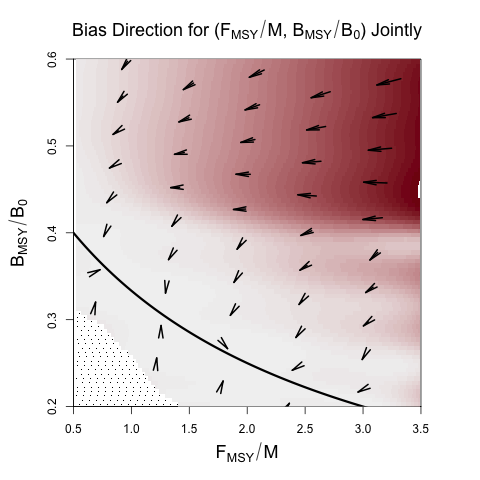
\includegraphics[width=0.32\textwidth]{../../ddBias/directionalBiasDDSubFlatT45N150A0-1AS0.1K10N56.png}
	%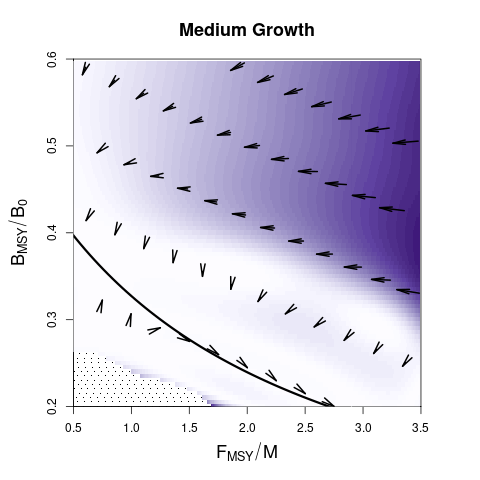
\includegraphics[width=0.32\textwidth]{../../ddBias/directionalBiasDDSubFlatT45N150A0-1AS1K0.5N56Purples.png} %directionalBiasDDSubFlatT45N150A0-1AS1K0.5N56.png}
	%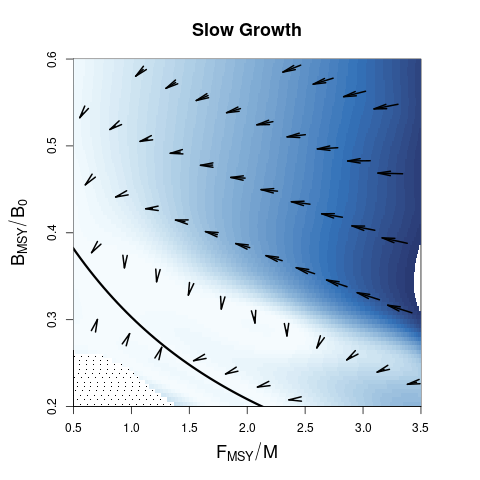
\includegraphics[width=0.32\textwidth]{../../ddBias/directionalBiasDDSubFlatT45N150A0-1AS2K0.1N84EdgeBlues.png}\\
	%%\end{minipage}
        %%\begin{minipage}[h!]{0.75\textwidth}
	%%{\color{red} 1\% \& 50\% Error Titles}\\
	%%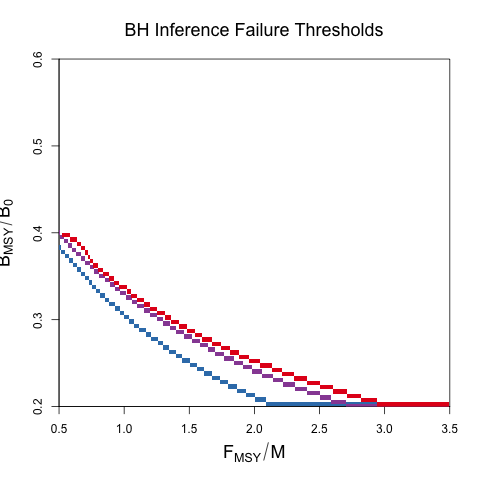
\includegraphics[width=0.49\textwidth]{../../ddBias/relErrorImagesBHDD0.01.png}
	%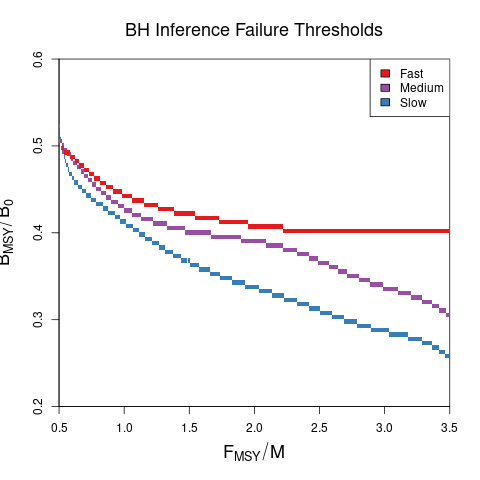
\includegraphics[width=\textwidth]{../../ddBias/relErrorImagesBHDD0.5.png}
	%%\end{minipage}

	%%
	%\begin{minipage}[h!]{0.3\textwidth}
	%
	%%BH is said to be estimating well when:
	%We want a small percent error in RP estimation:
	%\begin{align*}
	%\frac{\frac{F_{MSY}}{M}-\frac{\hat{F}_{MSY}}{M}}{\frac{F_{MSY}}{M}}\le P\\
	%%\end{align*}
	%%%%Or equivalently:
	%%\begin{align*}
	%\hat{F}_{MSY}\ge(1-P)F_{MSY}
	%\end{align*}
	%
	%%\hat y(\textbf{x}), \hat \sigma^2(\textbf{x})
	%Declare model failure when:
	%\begin{equation*}
	%e^{\hat y(\textbf{x}) + \sqrt{2\hat \sigma^2(\textbf{x})}\Phi^{-1}\left(\frac{1}{10}-1\right)}<(1-P)F_{MSY} 
	%\end{equation*}
	%
	%%
	%Catastrophic model failure is identified by taking $P$ to be 0.5. Hypotheses may be refined by reducing $P$ as relevant.
	%%{\color{red}Maybe more text? add $P=0.5$ in title? somewhere. Embigg}
	%
	%%
	%\end{minipage}
        %\begin{minipage}[h!]{0.74\textwidth}
	%	
	%	%
	%	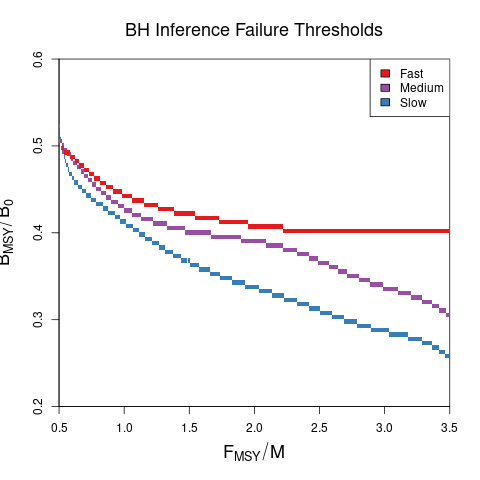
\includegraphics[width=0.24\textwidth]{../../ddBias/relErrorImagesBHDD0.5.png}	
	%	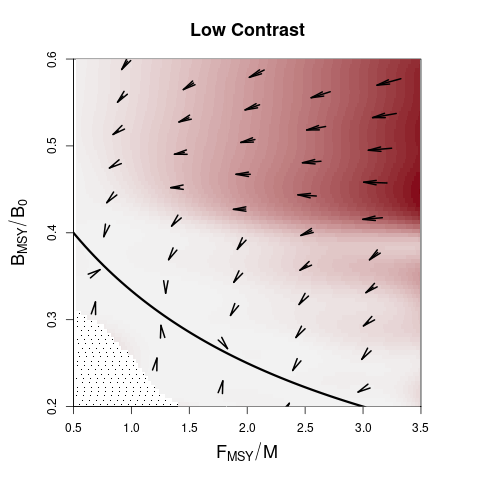
\includegraphics[width=0.24\textwidth]{../../ddBias/directionalBiasDDSubFlatT45N150A0-1AS0.1K10N56Reds 2.png}
	%	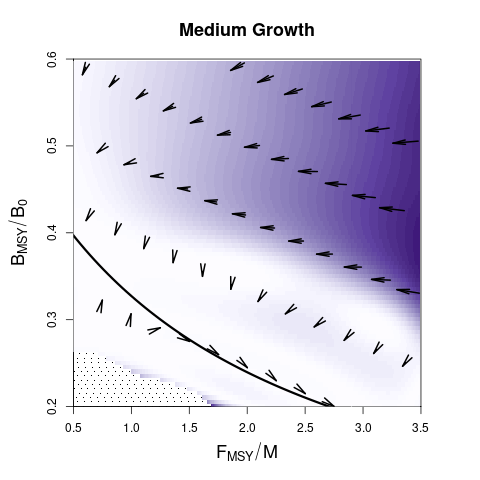
\includegraphics[width=0.24\textwidth]{../../ddBias/directionalBiasDDSubFlatT45N150A0-1AS1K0.5N56Purples.png}
	%	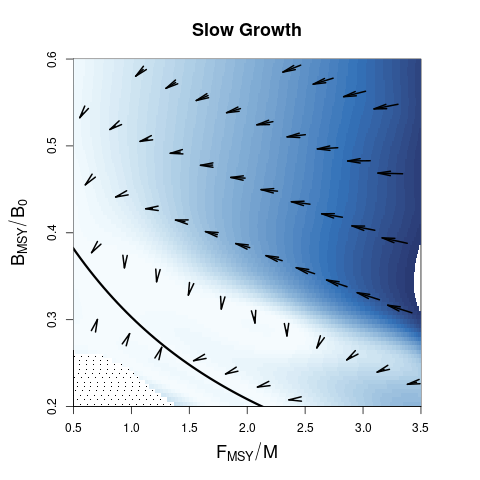
\includegraphics[width=0.24\textwidth]{../../ddBias/directionalBiasDDSubFlatT45N150A0-1AS2K0.1N84EdgeBlues.png}
	%	
	%	%%{\color{red}add $P=0.5$ in title? somewhere. Embiggen}\\	
        %	%\begin{minipage}[h!]{0.5\textwidth}
        %	%%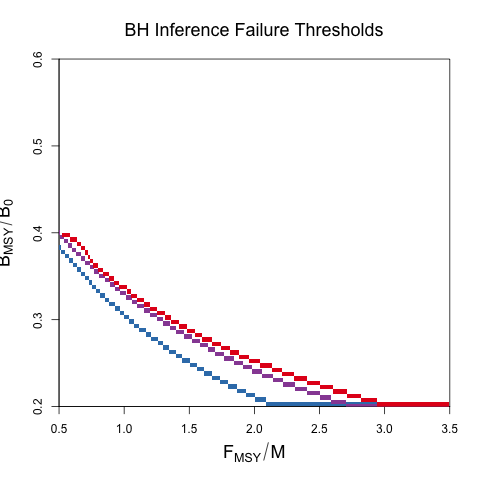
\includegraphics[width=0.49\textwidth]{../../ddBias/relErrorImagesBHDD0.01.png}
        %	%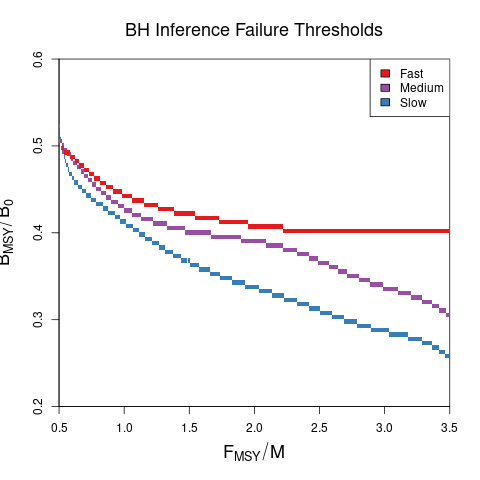
\includegraphics[width=\textwidth]{../../ddBias/relErrorImagesBHDD0.5.png}\\
	%	%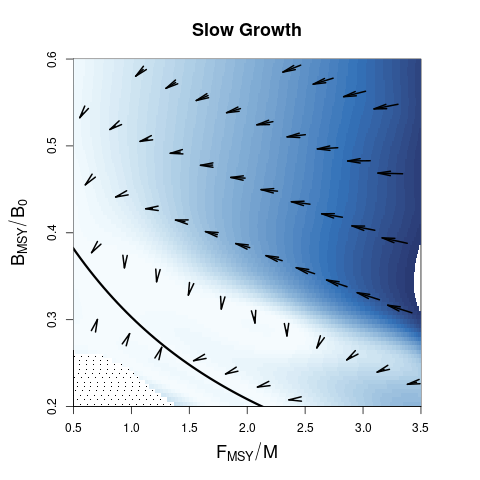
\includegraphics[width=\textwidth]{../../ddBias/directionalBiasDDSubFlatT45N150A0-1AS2K0.1N84EdgeBlues.png}	
	%	%\end{minipage}
	%	%\begin{minipage}[h!]{0.5\textwidth}
	%	%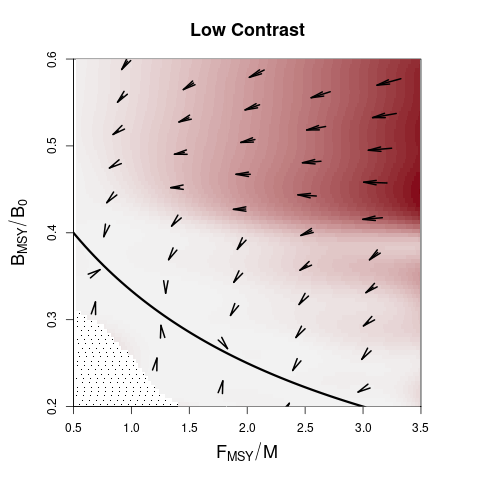
\includegraphics[width=\textwidth]{../../ddBias/directionalBiasDDSubFlatT45N150A0-1AS0.1K10N56Reds 2.png}\\
	%	%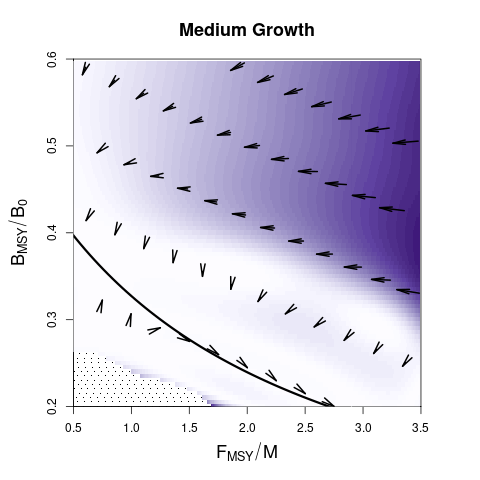
\includegraphics[width=\textwidth]{../../ddBias/directionalBiasDDSubFlatT45N150A0-1AS1K0.5N56Purples.png}
        %	%\end{minipage}	
	%	%%%{\color{red}add $P=0.5$ in title? somewhere. Embiggen}\\	
        %	%%\begin{minipage}[h!]{0.73\textwidth}
        %	%%%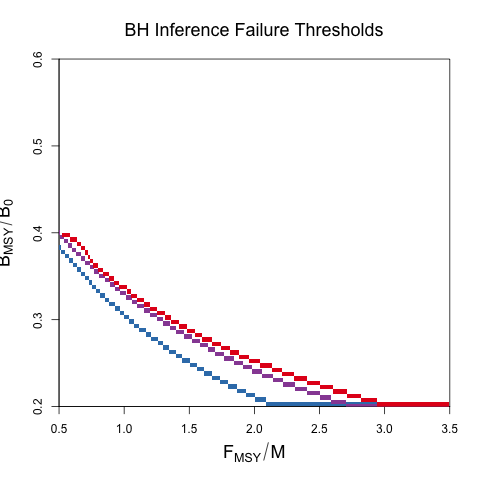
\includegraphics[width=0.49\textwidth]{../../ddBias/relErrorImagesBHDD0.01.png}
        %	%%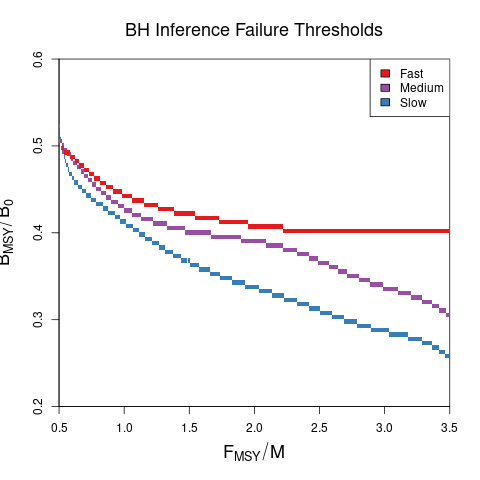
\includegraphics[width=\textwidth]{../../ddBias/relErrorImagesBHDD0.5.png}
	%	%%\end{minipage}
	%	%%\begin{minipage}[h!]{0.24\textwidth}
	%	%%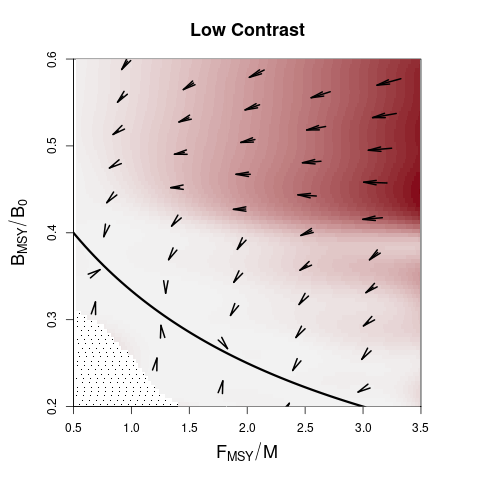
\includegraphics[width=\textwidth]{../../ddBias/directionalBiasDDSubFlatT45N150A0-1AS0.1K10N56Reds 2.png}\\
        %	%%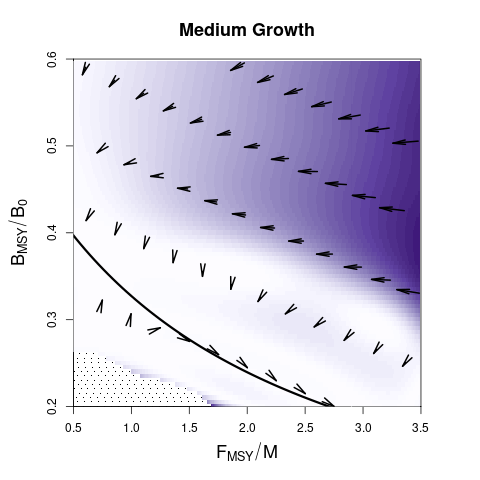
\includegraphics[width=\textwidth]{../../ddBias/directionalBiasDDSubFlatT45N150A0-1AS1K0.5N56Purples.png}\\
        %	%%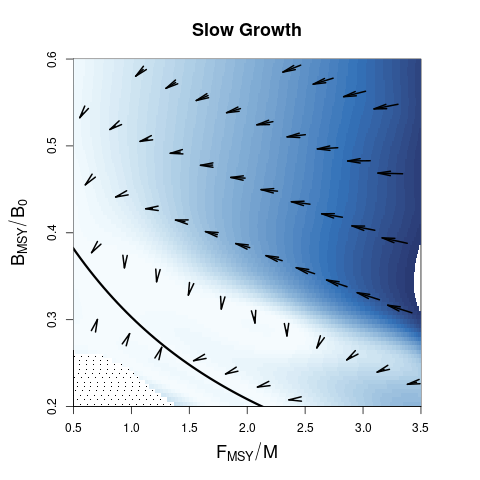
\includegraphics[width=\textwidth]{../../ddBias/directionalBiasDDSubFlatT45N150A0-1AS2K0.1N84EdgeBlues.png}
        %	%%\end{minipage}
	%\end{minipage}

	%
        \begin{minipage}[h!]{0.74\textwidth}
	%
	\raggedright
	Overall RPs are underestimated by the two-parameter model. When two-parameter model misspecification\\ 
	becomes ``large'' %datasets result in a heavily misspecified two-parameter model, 
	RPs are catastrophically underestimated. This breakpoint is a function of growth.\\$~$\\
	%	
	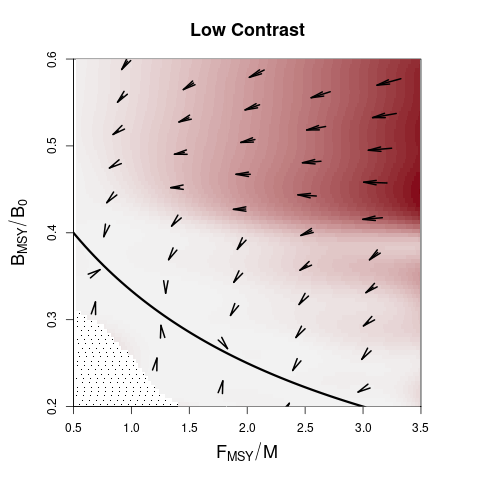
\includegraphics[width=0.24\textwidth]{../../ddBias/directionalBiasDDSubFlatT45N150A0-1AS0.1K10N56Reds 2.png}
	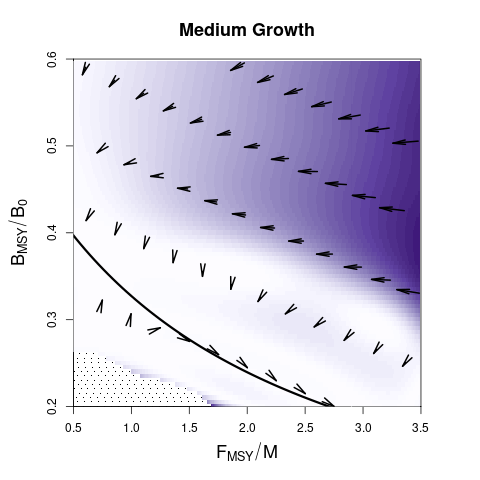
\includegraphics[width=0.24\textwidth]{../../ddBias/directionalBiasDDSubFlatT45N150A0-1AS1K0.5N56Purples.png}
	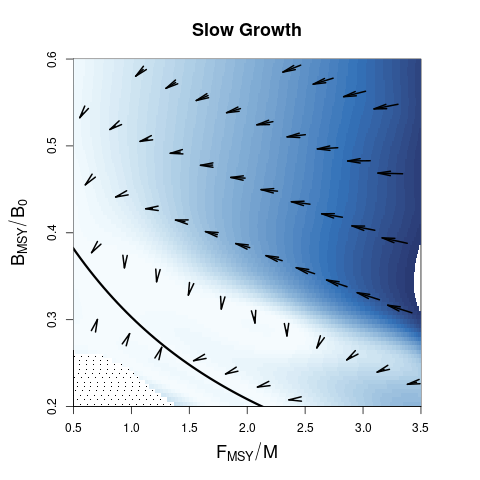
\includegraphics[width=0.24\textwidth]{../../ddBias/directionalBiasDDSubFlatT45N150A0-1AS2K0.1N84EdgeBlues.png}
	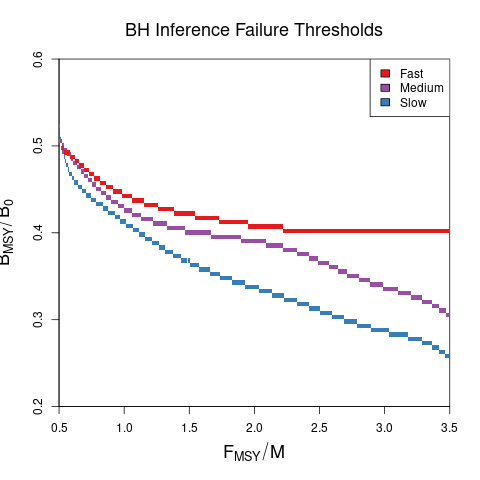
\includegraphics[width=0.24\textwidth]{../../ddBias/relErrorImagesBHDD0.5.png}	
	
	%
	\vspace{0.2cm}
	Since RPs are generally underestimated, a one-sided test used to idetify model failure. %considered. 
	Hypotheses may be refined by specifying $P$.
	Catastrophic model failure is identified by taking $P$ to be 0.5. 

	%
        \end{minipage}
        \begin{minipage}[h!]{0.26\textwidth}
	
	%
	The GP metamodel predicts the inferred RP mean $\hat y(\textbf{x})$ \& variance $\hat \sigma^2(\textbf{x})$ as a function the true RPs, %$\textbf{x}$,
	%
	%%complete with uncertainty%and variance $\hat \sigma^2(\textbf{x})$ 
	%as a function of the particular model mispecification $\textbf{x}$.
	%%estimates of BH RPs for  are obtained via kriging	
	%%%
	%%The GP full predictive description of inference
	%%under the misspecified restricted models.
	%%Predictive estimates are obtained via kriging
	%\vspace{-0.25cm}
        \begin{equation*}
        \log(\hat{F}_{MSY}) \sim N\Big(\hat y(\textbf{x}), \hat \sigma^2(\textbf{x})\Big).
        \end{equation*}
	%\vspace{-0.25cm}
	%BH is said to be estimating well when:
        We want a small percent error in RP estimation:
        \begin{align*}
        \frac{\frac{F_{MSY}}{M}-\frac{\hat{F}_{MSY}}{M}}{\frac{F_{MSY}}{M}}\le P\\
        %\end{align*}
        %%%Or equivalently:
        %\begin{align*}
        \hat{F}_{MSY}\ge(1-P)F_{MSY}
        \end{align*}

        %\hat y(\textbf{x}), \hat \sigma^2(\textbf{x})
        Declare model failure when:
        \begin{equation*}
        e^{\hat y(\textbf{x}) + \sqrt{2\hat \sigma^2(\textbf{x})}\Phi^{-1}\left(\frac{1}{10}-1\right)}<(1-P)F_{MSY} 
        \end{equation*}
	%Since RPs are generally underestimated only the one sided test is considered.
	%
        \end{minipage}
}

%%
%\headerbox{4. Conclusions}{name=conclusion,column=2,below=model,span=1}{
%	%
%	\begin{itemize}
%	\raggedright
%	\item[$~$]
%	\item A rich simulation-based method for describing global RP bias.
%	\item GP metamodel, describes and identifies breakpoints well in this setting. %despite sharp breakpoints.
%	
%	\item Two-parameter model largely under\\ estimates $\frac{F_{MSY}}{M}$.
%	\item As model misspecification becomes ``large'', RP estimation breaks\\ catastrophically.
%	\item Slower growth exaggerates model\\ misspecification. % relative to  model.
%	\item[$~$]
%	%%\item I love words.
%	%\item Words are hard.
%	%\item Even though they are hard, it's good to use them.
%	%\item Words are free and very powerful when used correctly.
%	\end{itemize}
%	
%	%$~$\\
%	%A Bayesian model-based method for speciating commercial landings shows promise. 
%	%BMA adds robustness to models by effectively integrating over modeling uncertainties.
%	%\\\\
%	%\underline{\textbf{Achievments of the Bayesian Approach:}}
%	%\begin{itemize}
%	%\item Model Overdispersion
%	%\item Robust Uncertainty Estimation
%	%\item Mechanisms for Pooling
%	%\item Out-of-Sample Predictions
%	%\end{itemize}
%	%$~$\\
%	%\underline{\textbf{Future Directions:}}
%	%\begin{itemize}
%	%\item Explore Additional Random Effects
%	%\item Possible Multivariate Likelihoods
%	%\item Dirichlet Process Models
%	%\end{itemize}
%	%\vspace{0.15cm}
%}
%
%%%
%%\headerbox{5. Another}{name=conclusion,column=2,below=conclusion,span=1}{
%%	Is there any reason to have another one down here?
%%	I fels like it could be nice, lets see?
%%}

%
\headerbox{References}{name=ref,column=0,below=cluster,span=3}{
	%{\renewcommand{\markboth}[2]{}}% Remove header adjustment
	%\printbibliography}
	%
	%\renewenvironment{thebibliography}[1]
     	%{\section*{\refname}{}%
	%
	%\renewenvironment{thebibliography}[1]
	%{\section*{\refname}{}%

	%\clearpage
	%\pagestyle{plain}
	%\bibliographystyle{plain}	
	%\bibliographystyle{apacite}
	%\bibliographystyle{IEEEtran}
	
	\begingroup
	\def\chapter*#1{}
	%\bibliographystyle{apacite}
	\bibliography{./gpBias.bib} %,./spline.bib,./spaceFilling.bib,./ageStructure.bib}
	\endgroup
	
	%\printbibliography[heading=none]	
}


%\headerbox{6. Conclusions}{name=conclusion,column=1,below=sea,span=2,above=bottom}{
%% DeCAF is a chemoinformatical tool that can be helpful in ligand-based drug design.
%% It provides a comprehensive molecule description and a fast algorithms for comparing and aligning multiple ligands.
%We proved that DeCAF is a significant improvement over the SEA algorithm, a popular method for comparing sets of ligands.
%\begin{boenumerate}\compresslist
%    \item DeCAF gives better results for 23 out of 35 receptors.
%    \item For targets with easily separable active and inactive datasets, SEA and DeCAF give similar results.
%    \item In cases in which SEA fails to identify active molecules, our method performs substantially better.
%\end{boenumerate}
%% It can be also used in other [procedures], such as database screening or drug repositioning.
%% DeCAF is written in Python and freely available at \textbf{\color{darkgreen}http://bitbucket.org/marta-sd/decaf}. 
%}
%
%
%\headerbox{7. References}{name=references,column=0,span=1,below=mcs,above=bottom}{
%
%
%%\small % Reduce the font size in this block
%\renewcommand{\section}[2]{\vskip 0.05em} % Get rid of the default "References" section title
%%\nocite{*} % Insert publications even if they are not cited in the poster
%
%
%\bibliographystyle{unsrt}
%\bibliography{poster} % Use sample.bib as the bibliography file
%}

\end{poster}

\end{document}

